%A LaTeX model for SYSU General Phys. Lab. by Probfia Gao.
%用XeLaTeX编译
\documentclass[11pt,a4paper]{ctexart}

%在下面补全实验名,例如 实验BB3 光电效应实验。
\newcommand{\ExpeName}{实验CA1 密立根油滴实验}

\usepackage{fancyhdr}
\usepackage{amsmath}
\usepackage{graphicx}
\usepackage[hmargin=1.25in,vmargin=1in]{geometry}
\usepackage{pdfpages}
\usepackage[colorlinks,
            linkcolor=red,
		 urlcolor=black]{hyperref}
\usepackage{cleveref}
\usepackage{amssymb}

\crefname{equation}{}{}
\crefname{figure}{图}{图}
\crefname{footnote}{注释}{注释}

%\cpic{<尺寸>}{<文件名>}}用于生成居中的图片。
\newcommand{\cpic}[2]{
\begin{center}
\includegraphics[scale=#1]{#2}
\end{center}
}

%\cpicn{<尺寸>}{<文件名>}{<注释>}用于生成居中且带有注释的图片,其label为图片名。
\newcommand{\cpicn}[3]
{
\begin{figure}[h!]
\cpic{#1}{#2}
\caption{#3\label{#2}}
\end{figure}
}

\newcommand{\beq}{\begin{equation}}
\newcommand{\eeq}{\end{equation}}
\newcommand{\bea}{\begin{equation}\begin{aligned}}
\newcommand{\eea}{\end{aligned}\end{equation}}

%输入单位和数学常数
%下面所有命令需在公式环境下使用
\newcommand{\e}{\mathrm{\ e}}   %自然常数e = \e
\newcommand{\im}{\mathrm{\ i}}   %虚数单位i = \im
\newcommand{\meter}{\mathrm{\ m}}      %单位/前缀 = \单位/前缀英文名
\newcommand{\newton}{\mathrm{\ N}}  
\newcommand{\joule}{\mathrm{\ J}}
\newcommand{\second}{\mathrm{\ s}}
\newcommand{\gram}{\mathrm{\ g}}
\newcommand{\ampere}{\mathrm{\ A}}
\newcommand{\kilogram}{\mathrm{\ kg}}
\newcommand{\kelvin}{\mathrm{\ K}}
\newcommand{\mole}{\mathrm{\ mol}}
\newcommand{\volt}{\mathrm{\ V}}
\newcommand{\degreeC}{\ ^\circ \mathrm{C}}  %摄氏度符号 = \degreeC



\pagestyle{fancy}

\fancyhead[L]{\footnotesize{中山大学物理与天文学院基础物理实验}}
\fancyhead[R]{\footnotesize{\ExpeName}}
\fancyfoot[C]{\thepage}

\begin{document}
%第一页
\cpic{0.255}{e1}%学生信息和计分表格
\begin{center}
\LARGE\textbf{{\ExpeName}}
\end{center}
\large{【实验报告注意事项】}
\begin{enumerate}
 \item 实验报告由三部分组成:
 \begin{enumerate}
  \item[1)]预习报告:(提前一周)认真研读\textbf{\uline{实验讲义}},弄清实验原理;实验所需的仪器设备、用具及其使用(强烈建议到实验室预习),完成讲义中的预习思考题;了解实验需要测量的物理量,并根据要求提前准备实验记录表格(由学生自己在实验前设计好,可以打印)。预习成绩低于10分(共20分)者不能做实验。
  \item[2)]实验记录:认真、客观记录实验条件、实验过程中的现象以及数据。实验记录请用珠笔或者钢笔书写并签名({\color{red}用铅笔记录的被认为无效})。{\color{red}保持原始记录,包括写错删除部分,如因误记需要修改记录,必须按规范修改。}(不得输入电脑打印,但可扫描手记后打印扫描件);离开前请实验教师检查记录并签名。
  \item[3)]分析讨论:处理实验原始数据(学习仪器使用类型的实验除外),对数据的可靠性和合理性进行分析;按规范呈现数据和结果(图、表),包括数据、图表按顺序编号及其引用;分析物理现象(含回答实验思考题,写出问题思考过程,必要时按规范引用数据);最后得出结论。
 \end{enumerate}
 \textbf{实验报告}就是预习报告、实验记录、和数据处理与分析合起来,加上本页封面。
 \item 每次完成实验后的一周内交\textbf{实验报告}。
 \item 除实验记录外,实验报告其他部分建议双面打印。
\end{enumerate}
\ 
\\
\ 

\begin{flushright}                                                           %模板作者
\tiny{
A \LaTeX \ model for General Phys. Lab., SPA, SYSU by {\em \href{https://www.weibo.com/3532532974/profile?rightmod=1&wvr=6&mod=personinfo&is_all=1}{Probfia} Gao.}\\ Adopted from the \href{http://lovephysics.sysu.edu.cn/lib/exe/fetch.php?media=courses:secondlevelzhuhai:report.docx}{original MS Word model} on \href{http://lovephysics.sysu.edu.cn}{Lovephysics}.\\ You can view it on \href{https://github.com/Probfia/SYSU_GPL_C}{Github}.}
\end{flushright}

\newpage%预习报告
\begin{center}
\LARGE{\textbf{\ExpeName}}
\end{center}
\textbf{【实验目的】}
\begin{enumerate}
 \item[1.] 学习用油滴实验测量电子电荷的原理。
 \item[2.] 利用静态法和动态法观测带电油滴的运动状态,测量不同带电油滴的电荷量,验证电荷的不连续性,测量电子电荷值$e$。
 \item[3.] 了解CCD摄像机、光学系统的成像原理,了解显微测量方法以及视频信号处理技术的工程应用等。
\end{enumerate}
\textbf{【仪器用具】}
%将讲义中的表格截图保存为t1在该文件夹下后删去下一行之前的%符号,合理调整scale参数。
\cpic{0.3}{t1}
%或者自己去 https://www.tablesgenerator.com/ 做一个表。
\textbf{【原理概述】}\par
该实验测量元电荷$e$的值,用到的方法著名的密立根油滴法。具体而言,实验有两种方法测量元电荷的值。
\par
第一种方法称为静态平衡法,它利用了油滴重力与电场力或空气阻力的平衡(浮力忽略不计)。油滴在无电场的空气中匀速下落的平衡方程是
\beq \label{1steq}
\frac{4\pi}{3}r^3 \rho_o g = 6\pi \frac{\eta}{1 + b/p r} \frac{L}{t_g}
\eeq
从中解得半径$r$和油滴质量$m$。再调整电压,使得电场力和重力能够平衡
\beq
mg = \frac{qU}{L}
\eeq
以上两式联立就可以得到电荷量的表达式
\beq \label{staq}
q = \frac{18\pi}{\sqrt{2\rho_0 g}}[\frac{\eta L}{t_g (1 + b/p r)}]^{3/2} \frac{d}{U} \\
\eeq
其中
\beq
r = \sqrt{\frac{9\pi v_g}{2\rho_o g}}
\eeq
\par
第二种方法称为动态法,它利用油滴在无电场下匀速下降和较强电场下匀速上升的速度比测量电荷量。油滴上升时的速度$v_e$满足平衡方程
\beq
6\pi r \eta v_e = q\frac{U}{d} - mg
\eeq
带入之前得到的$v_g = \cfrac{L}{t_g}$和$m$的表达式即得
\beq \label{dynq}
q = \frac{18\pi}{\sqrt{2\rho_0 g}}[\frac{\eta L}{t_g (1 + b/p r)}]^{3/2} \frac{d}{U} (\frac{1}{t_e} +\frac{1}{t_g}) \frac{1}{\sqrt{t_g}}
\eeq
令$t_e \to \infty$上式恢复到静态法的公式。
\\
\ 
\\
\textbf{【实验前思考题】}
\begin{enumerate}
 \item[1.] \textbf{密立根利用油滴测定电子电荷的基本原理是什么?}\par
就是力的平衡原理,别无他尔。
 \item[2.] \textbf{什么是静态(平衡)测量法和动态(非平衡)测量法?两种方法有何不同与优缺点?测量中需注意哪些问题?}\par
关于两种方法的概念见【原理概述】部分(公式\cref{1steq}到\cref{dynq})。静态法测量精度较高,但调整油滴处于静止状态较为不易;动态法对油滴的运动状态的限制较弱,从而降低了操作难度,但因为匀速上升很难精确达到,精度不如静态法。测量时需要注意安全,精密调节仪器的位置和参数。
\item[3.] \textbf{为什么必须保证油滴在测量范围内做匀速运动或静止?怎样控制油滴运动?}\par
因为实验的测量原理就是力的平衡原理,所以当然需要油滴达到匀速运动或静止状态。油滴运动通过控制平衡电压来实现。
\end{enumerate}

\newpage%实验记录
\iffalse
\cpic{0.255}{e2}%学生信息表格
\begin{center}
\LARGE{\textbf{\ExpeName}}
\end{center}
\textbf{【实验内容、步骤、结果】}\\
1. \textbf{调整和熟练仪器的使用}\par
按照讲义要求,调整仪器,学习控制油滴在视场中的运动。
\\
\ 
\\
2. \textbf{平衡法测量油滴所带的电荷量}\par
按照讲义要求,记录5个油滴的实验数据如下:
\begin{table}[h!]
\centering
\caption{平衡法测量第一个油滴的实验数据}
\label{my-label}
\begin{tabular}{|c|p{12mm}|p{12mm}|p{12mm}|p{12mm}|p{12mm}|p{12mm}|}
\hline
实验次数 & 1 & 2 & 3 & 4 & 5 & 平均值 \\ \hline
平衡电压/V &  &  &  &  &  &  \\ \hline
下落时间/s &  &  &  &  &  &  \\ \hline
电荷量/$10^{-19}\mathrm{\ C}$ &  &  &  &  &  &  \\ \hline
\end{tabular}
\end{table}
\begin{table}[h!]
\centering
\caption{平衡法测量第二个油滴的实验数据}
\label{my-label}
\begin{tabular}{|c|p{12mm}|p{12mm}|p{12mm}|p{12mm}|p{12mm}|p{12mm}|}
\hline
实验次数 & 1 & 2 & 3 & 4 & 5 & 平均值 \\ \hline
平衡电压/V &  &  &  &  &  &  \\ \hline
下落时间/s &  &  &  &  &  &  \\ \hline
电荷量/$10^{-19}\mathrm{\ C}$ &  &  &  &  &  &  \\ \hline
\end{tabular}
\end{table}
\begin{table}[h!]
\centering
\caption{平衡法测量第三个油滴的实验数据}
\label{my-label}
\begin{tabular}{|c|p{12mm}|p{12mm}|p{12mm}|p{12mm}|p{12mm}|p{12mm}|}
\hline
实验次数 & 1 & 2 & 3 & 4 & 5 & 平均值 \\ \hline
平衡电压/V &  &  &  &  &  &  \\ \hline
下落时间/s &  &  &  &  &  &  \\ \hline
电荷量/$10^{-19}\mathrm{\ C}$ &  &  &  &  &  &  \\ \hline
\end{tabular}
\end{table}
\newpage
\begin{table}[h!]
\centering
\caption{平衡法测量第四个油滴的实验数据}
\label{my-label}
\begin{tabular}{|c|p{12mm}|p{12mm}|p{12mm}|p{12mm}|p{12mm}|p{12mm}|}
\hline
实验次数 & 1 & 2 & 3 & 4 & 5 & 平均值 \\ \hline
平衡电压/V &  &  &  &  &  &  \\ \hline
下落时间/s &  &  &  &  &  &  \\ \hline
电荷量/$10^{-19}\mathrm{\ C}$ &  &  &  &  &  &  \\ \hline
\end{tabular}
\end{table}
\begin{table}[h!]
\centering
\caption{平衡法测量第五个油滴的实验数据}
\label{my-label}
\begin{tabular}{|c|p{12mm}|p{12mm}|p{12mm}|p{12mm}|p{12mm}|p{12mm}|}
\hline
实验次数 & 1 & 2 & 3 & 4 & 5 & 平均值 \\ \hline
平衡电压/V &  &  &  &  &  &  \\ \hline
下落时间/s &  &  &  &  &  &  \\ \hline
电荷量/$10^{-19}\mathrm{\ C}$ &  &  &  &  &  &  \\ \hline
\end{tabular}
\end{table}
\vspace{1cm}
\noindent 3. \emph{(选做)}\textbf{用动态法测量油滴所带的电荷量}\par
按照讲义要求,记录5个油滴的实验数据如下:
\begin{table}[h!]
\centering
\caption{动态法测量第一个油滴的实验数据}
\label{my-label}
\begin{tabular}{|c|p{12mm}|p{12mm}|p{12mm}|p{12mm}|p{12mm}|p{12mm}|}
\hline
实验次数 & 1 & 2 & 3 & 4 & 5 & 平均值 \\ \hline
提升电压/V &  &  &  &  &  &  \\ \hline
下落时间/s &  &  &  &  &  &  \\ \hline
提升时间/s &  &  &  &  &  &  \\ \hline
电荷量/$10^{-19}\mathrm{\ C}$ &  &  &  &  &  &  \\ \hline
\end{tabular}
\end{table}
\begin{table}[h!]
\centering
\caption{动态法测量第二个油滴的实验数据}
\label{my-label}
\begin{tabular}{|c|p{12mm}|p{12mm}|p{12mm}|p{12mm}|p{12mm}|p{12mm}|}
\hline
实验次数 & 1 & 2 & 3 & 4 & 5 & 平均值 \\ \hline
提升电压/V &  &  &  &  &  &  \\ \hline
下落时间/s &  &  &  &  &  &  \\ \hline
提升时间/s &  &  &  &  &  &  \\ \hline
电荷量/$10^{-19}\mathrm{\ C}$ &  &  &  &  &  &  \\ \hline
\end{tabular}
\end{table}
\begin{table}[h!]
\centering
\caption{动态法测量第三个油滴的实验数据}
\label{my-label}
\begin{tabular}{|c|p{12mm}|p{12mm}|p{12mm}|p{12mm}|p{12mm}|p{12mm}|}
\hline
实验次数 & 1 & 2 & 3 & 4 & 5 & 平均值 \\ \hline
提升电压/V &  &  &  &  &  &  \\ \hline
下落时间/s &  &  &  &  &  &  \\ \hline
提升时间/s &  &  &  &  &  &  \\ \hline
电荷量/$10^{-19}\mathrm{\ C}$ &  &  &  &  &  &  \\ \hline
\end{tabular}
\end{table}
\newpage
\begin{table}[h!]
\centering
\caption{动态法测量第四个油滴的实验数据}
\label{my-label}
\begin{tabular}{|c|p{12mm}|p{12mm}|p{12mm}|p{12mm}|p{12mm}|p{12mm}|}
\hline
实验次数 & 1 & 2 & 3 & 4 & 5 & 平均值 \\ \hline
提升电压/V &  &  &  &  &  &  \\ \hline
下落时间/s &  &  &  &  &  &  \\ \hline
提升时间/s &  &  &  &  &  &  \\ \hline
电荷量/$10^{-19}\mathrm{\ C}$ &  &  &  &  &  &  \\ \hline
\end{tabular}
\end{table}
\begin{table}[h!]
\centering
\caption{动态法测量第五个油滴的实验数据}
\label{my-label}
\begin{tabular}{|c|p{12mm}|p{12mm}|p{12mm}|p{12mm}|p{12mm}|p{12mm}|}
\hline
实验次数 & 1 & 2 & 3 & 4 & 5 & 平均值 \\ \hline
提升电压/V &  &  &  &  &  &  \\ \hline
下落时间/s &  &  &  &  &  &  \\ \hline
提升时间/s &  &  &  &  &  &  \\ \hline
电荷量/$10^{-19}\mathrm{\ C}$ &  &  &  &  &  &  \\ \hline
\end{tabular}
\end{table}
%\newline
\textbf{【实验过程中遇到问题记录】}
\fi

%生成最终报告时将上面内容全部删除或注释(用\iffalse \fi),将扫描得到的实验报告保存为Record.pdf在LaTeX model for GPL下,将下行命令的注释号删去。注意根据实际页数调整pages参数。
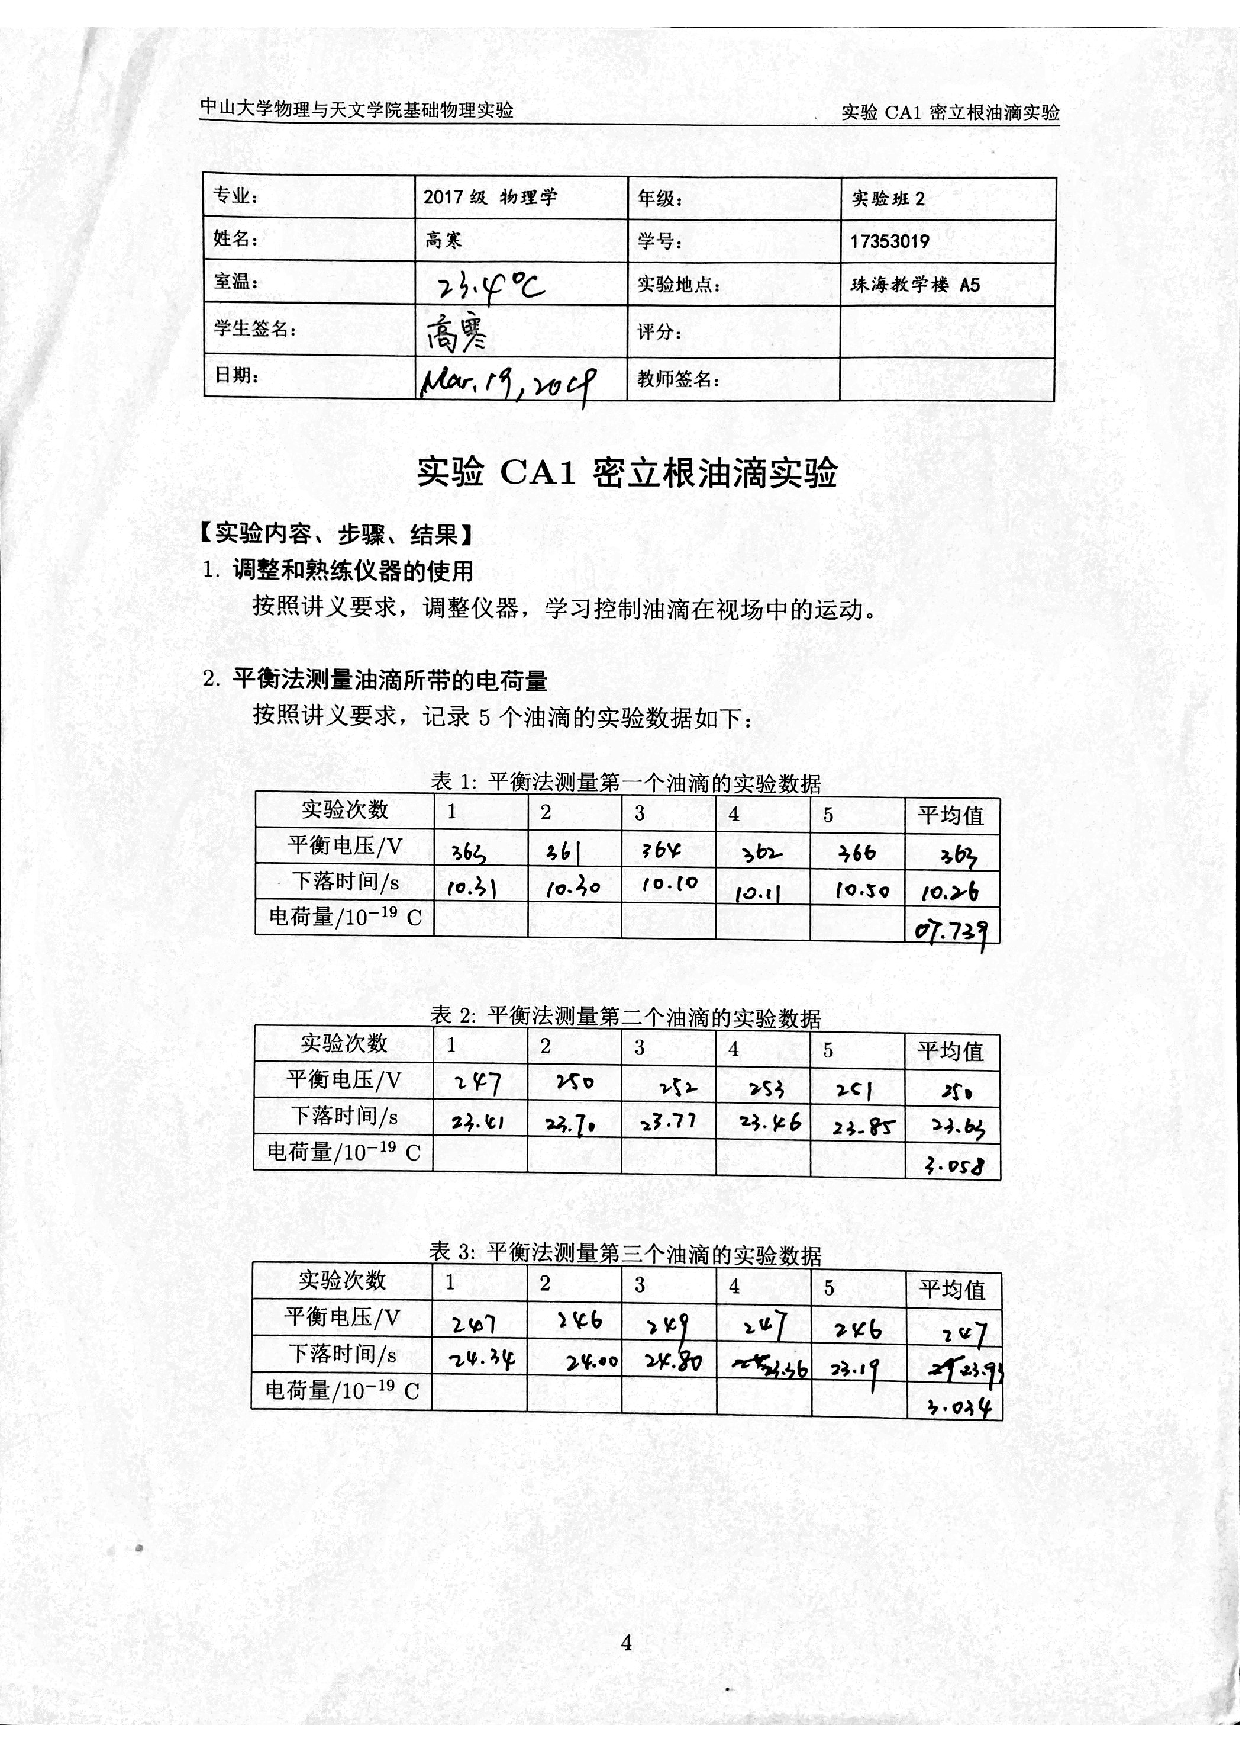
\includepdf[pages=1-3]{record}

\newpage%分析与讨论
\cpic{0.255}{e3}%学生信息表格
\begin{center}
\LARGE\textbf{{\ExpeName}}
\end{center}
\textbf{【分析与讨论】}\par
\newcommand{\charge}{\times 10^{-19}\mathrm{\ C}}

%\begin{document}

1. \textbf{平衡法测油滴所带的电荷量}\par
实验共测量了5颗油滴,它们的带电量由仪器用公式直接算出,为
\begin{gather}
	q_1 = 7.739 \charge \\
	q_2 = 3.058 \charge \\
	q_3 = 3.024 \charge \\
	q_4 = 13.680 \charge \\
	q_5 = 4.718 \charge
\end{gather}
用元电荷的估计值$1.6 \charge$来除以上面的电荷量,得到每个油滴的所带的净电子数为
\begin{gather}
	n_1 = \frac{7.739}{1.6} = 4.84 \simeq 5\\
	n_2 = \frac{3.058}{1.6} = 1.91 \simeq 2\\
	n_3 = \frac{3.024}{1.6} = 1.89 \simeq 2\\
	n_4 = \frac{13.680}{1.6} = 8.55 \simeq 9\\
	n_5 = \frac{4.718}{1.6} = 2.95 \simeq 3
\end{gather}
我们先不论$n_4$接近半整数的取值,而先将其简单地四舍五入进行元电荷的计算。5颗油滴各自代表的元电荷测量值为
\begin{gather}
	e_1 = \frac{7.739\charge}{5} = 1.548\charge\\
	e_2 = \frac{3.058\charge}{2} = 1.529\charge\\
	e_3 = \frac{3.024\charge}{2} = 1.512\charge\\
	e_4 = \frac{13.680\charge}{9} = 1.520\charge\\
	e_5 = \frac{4.718\charge}{3} 1.553\charge
\end{gather}
综合测量结果,得到元电荷的测量平均值为
\bea
	e &= \frac{1.548+1.529+1.512+1.52+1.573}{5}\charge  \\
	&= 1.532\charge
\eea
平均值的标准偏差为实验误差,其值计算为
\bea
	\sigma_e &= \frac{1}{\sqrt{5}} (\frac{1}{5-1}[(1.548-1.536)^2 +(1.529-1.536)^2 +(1.512-1.536)^2  \\ 
&+(1.52-1.536)^2 +(1.573-1.536)^2 ])^{\frac{1}{2}} \charge \\
	&= 0.007\charge
\eea
综合测量值表示为
\beq
	e = (1.532 \pm 0.007)\charge
\eeq
与实际值$e = 1.602 \charge$的相对误差为
\beq
\delta_e = \frac{1.602 - 1.549}{1.602} = 4.3\%
\eeq
以标准差衡量的距离为
\beq
\frac{1.602-1.532}{0.007} = 10
\eeq
这个值远高于$3$,说明了系统误差的存在。
\par
我们发现,不论是看单个数值,还是看整体的综合数据,测量得到的$e$都是偏小的。仪器可能存在一定的系统误差,误差的来源可能是因为实验参数的设置偏差(例如大气压和重力加速度);仪器本身的制造偏差(例如极板间的距离可能与预设值有所偏差,或电压的显示值偏大)。
\par
我们发现,测量出半整数电荷不是因为别的,就是因为这个油滴的带电量较大,而对单个元电荷测量的误差是相当的;这些相当的误差累计,导致了恰好累计出了半个元电荷的差距。事实上,用这颗电荷测量出的$e$值落在综合测量值的$3\sigma$范围内,因此,半整数电荷不是别的,就是误差的累计。用实验得到的元电荷值计算它的电子数就是一个整数。
\par
\cpicn{0.4}{fitstat}{静态法测量的$(n_i,q_i)$散点图和回归直线}
另一种数据处理方法是作$(n_i,q_i)$散点图求出回归直线的斜率为元电荷值,散点图如\cref{fitstat}

其回归直线的斜率为
\beq
e = (1.52 \pm 0.02)\charge
\eeq
这个处理方法带来的标准偏差和相对标准值的误差都更大。
\\
\par
2.\textbf{动态法测油滴所带的电荷量}\par
对于动态法,实验同样测量了5颗不同油滴,并由仪器直接给出电荷量,分别为
\begin{gather}
	q_1 = 6.309 \charge \\
	q_2 = 3.103 \charge \\
	q_3 = 3.051 \charge \\
	q_4 = 3.073 \charge \\
	q_5 = 1.553 \charge
\end{gather}
它们所带的净电子数估计值为
\begin{gather}
	n_1 = \frac{6.309}{1.6} = 3.94 \simeq 4\\
	n_2 = \frac{3.103}{1.6} = 1.94 \simeq 2\\
	n_3 = \frac{3.051}{1.6} = 1.91 \simeq 2\\
	n_4 = \frac{3.073}{1.6} = 1.92 \simeq 2\\
	n_5 = \frac{1.553}{1.6} = 0.97 \simeq 1
\end{gather}
各个$n_i$的值都较接近的整数要小一些,依然体现出了系统误差的存在。同样的方法处理各个油滴的实验数据,得到它们各自代表的元电荷测量值为
\begin{gather}
	e_1 = \frac{6.309\charge}{4} = 1.578\charge\\
	e_2 = \frac{3.103\charge}{2} = 1.552\charge\\
	e_3 = \frac{3.051\charge}{2} = 1.526\charge\\
	e_4 = \frac{3.073\charge}{2} = 1.537\charge\\
	e_5 = \frac{1.553\charge}{1} = 1.553\charge
\end{gather}
平均值为
\bea
	e &= \frac{1.578+1.552+1.526+1.537+1.553}{5}\charge  \\ &= 1.549\charge
\eea
平均值的标准偏差为
\bea
\sigma_e &= \frac{1}{\sqrt{5}} (\frac{1}{5-1}[(1.578-1.549)^2 +(1.552-1.549)^2 +(1.526-1.549)^2 \\
&+(1.537-1.549)^2 +(1.553-1.549)^2 ])^{\frac{1}{2}} \charge \\
&= 0.008\charge
\eea
综合测量值表示为
\beq
	e = (1.549 \pm 0.008)\charge
\eeq

与真实值的相对误差为
\beq
\delta_e = \frac{1.602-1.549}{1.602} = 3.3\%
\eeq
以标准差衡量的距离为
\beq
\frac{1.602-1.549}{0.008} = 6.6
\eeq
\cpicn{0.4}{fitdyna}{动态法测量的$(n_i,q_i)$散点图和回归直线}
这个误差虽然比静态法要好,但也超过了$3\sigma$的极限误差范围,说明了系统误差的存在。我们发现,动态法测量带来的随机误差稍大,但与真实值的相对误差却稍小。
\par

同样用回归直线方法再次处理实验数据,得到的散点图和回归直线如\cref{fitdyna},其斜率为
\beq
e = (1.59 \pm 0.02)\charge
\eeq
虽然这个数据处理方法带来了较大的标准偏差,但它确十分接近标准值,且误差落在$1\sigma$的范围内。
\par
理论上讲,用回归直线方法处理数据更为合理,假如对电荷的测量存在一个固定的,与电荷量无关的系统误差的话,用回归直线计算可以将这个误差归结到直线的截距上,从而消除这部分误差。
\par
综合上面四个测量结果,将它们视作不等精度列,得到综合测量结果为
\bea
e &= \frac{1.532/0.007^2 + 1.52/0.02^2 + 1.549/0.008^2 + 1.59/0.02^2}{1/0.007^2 + 1/0.02^2 + 1/0.008^2 + 1/0.02^2} \charge \\
&= 1.541\charge
\eea
综合不确定度
\beq
\sigma_e = \sqrt{\frac{1}{1/0.007^2 + 1/0.02^2 + 1/0.008^2 + 1/0.02^2}} = 0.005\charge
\eeq
故,这次实验的最终结果为
\beq
e = (1.541 \pm 0.005)\charge
\eeq
\newpage
\textbf{【实验思考题】}\par
\begin{enumerate}
\item \textbf{试分析本实验的主要误差来源。}\par
本实验的主要误差来源可分为系统误差和偶然误差两大类,系统误差可能来源于:
\begin{enumerate}
\item 参数的设定,例如大气压与重力加速度,与当地的真实值存在差异;
\item 电压或极板距离的测量与真实值不符,或两极板间的电场在平衡位置不能视为匀强电场;
\item 忽略了油滴下落和上升时做加速运动的过程。
\end{enumerate}
偶然误差主要来源于:
\begin{enumerate}
\item 计时由于人反应时间的存在,对那些下落速度极快的油滴(通常是较大的油滴),会带来极大的偶然误差;
\item 油滴的布朗运动或飘动使得电荷下落的时间偏大,在实验中事实上观察到油滴有时会做很明显的水平飘动;
\item 油滴的平衡有时难以判断,很多时候,小幅度地调整电压对油滴的运动或平衡状态没有显著的影响。
\end{enumerate}
\item \textbf{在完成自己实验数据分析的基础上,把本实验班(约 12 名)同学的数据做统计分析,并与电子电荷值比较。}
\item \textbf{密立根油滴实验的总结(油滴筛选、跟踪、测量……)(经验分享;体会;感想;讨论;建议等)。}\par
分以下几点讲:
\begin{enumerate}
\item 油滴筛选时千万不要选择过大的油滴,否则它的下落会非常快。通常线度为2-3个显示器上刻度线宽度的油滴较为合适;
\item 在选择油滴时可以先设定好一个平衡电压,并保持它在工作状态下喷入油滴,等待一段时间,平衡电压在预设值附近的油滴自然会留着视野范围内;
\item 这个实验给我带来的体会是,选对仪器很重要;
\item 这个实验给我的感想是,虽然这个实验在整个物理学史上的地位非常重要,但是这个实验好无聊;
\end{enumerate}
\item \emph{(选做)}\textbf{在实验原理中,我们是把油滴作为一个孤立的带电球来进行处理的,也就是说,我们忽略了油滴之间的相互作用(静电排斥),或其他油滴所带电荷对所观察的油滴附近电场所造成的影响。那么,在什么样的情况下,这种近似的考虑才可以成立。}\par
设整个电场区域的体积为$V=Al$,油滴的数目为$N$,板间电压为$U$,间距为$l$,于是油滴间的间距大概是
\beq
s \simeq \sqrt[3]{\frac{Al}{N}}
\eeq
每个油滴带电量大约是$\sim e$的量级,它在相邻油滴的位置产生的场强大概为
\bea
E_o &\sim \frac{1}{4\pi \epsilon_0} \frac{e}{s^2} \\
&\sim \frac{1}{4\pi \epsilon_0} e (\frac{N}{Al})^{2/3}
\eea
而板间电场的大小是
\beq
E = \frac{U}{l}
\eeq
近似成立的条件是
\beq
E_o \lesssim E
\eeq
再假设$A \sim l^2$,带入化简得
\beq
N \lesssim  (\frac{4\pi \epsilon_0 Ul}{e})^{3/2}
\eeq
由$4\pi \epsilon_0 = \cfrac{1}{9\times 10^9} \mathrm{\ C^2/(N\cdot m^2)}$,$e = 1.6\charge$,$l = 5\mathrm{\ mm}$,$U \sim 200\volt$,得到近似成立的条件
\bea
N &\lesssim (\frac{200\times 0.005}{9\times 10^9 \times 1.6\times 10^{-19}})^{3/2} \\
&\simeq (\frac{1}{1.5\times 10^{-6}})^{3/2} \\
&\simeq 10^9
\eea
但真正选择合适的油滴开始测量时,由简单的幼儿园数学可以数出来电场区域间的油滴数仅有$N \sim 1$量级,故这个近似是符合地非常好的。


\end{enumerate}




\end{document}